\chapter{Visual Receptive Fields}
\label{ch:receptive-fields}

\textit{A receptive field is a linear map from stimulus space to response. This chapter develops that map for simple cells, then shows how Gabor structure, space-time separability, and the energy model explain selectivity, direction tuning, and phase invariance.}

% ============================================================
\section{Receptive Fields and the Linear Model}
\label{sec:receptive-field}
% ============================================================

The \emph{receptive field}\index{receptive field} of a visual neuron is the region of the visual field that influences its firing. Hubel and Wiesel's\index{Hubel and Wiesel} classic experiments showed that neurons in primary visual cortex (V1) respond selectively to oriented bars and edges at particular positions. A vertical bar might drive a neuron strongly, while a horizontal bar at the same location produces no response at all. The neuron's tuning curve---its firing rate as a function of stimulus orientation---has a clear peak at its preferred angle.

The simplest quantitative model treats the neuron as a \emph{linear filter}\index{linear filter} acting on the visual stimulus. The stimulus $s(x, y, t)$ is a function of space and time (the light intensity at each point in the visual field at each moment). The neuron's response at time $t$ is a weighted integral over recent stimulus history:

\begin{keyequation}[Linear Receptive Field Model]
\begin{equation}
  L(t) = \int_0^\infty \!\dd\tau \iint \dd x\,\dd y\; D(x, y, \tau)\, s(x, y, t - \tau)
  \label{eq:linear-rf}
\end{equation}
\tcblower
$L(t)$: linear response, \quad
$D(x, y, \tau)$: space-time receptive field kernel, \quad
$s$: stimulus.
\end{keyequation}

\noindent This is a convolution: the kernel $D(x, y, \tau)$ tells us how much weight the neuron gives to stimulus at position $(x, y)$ presented $\tau$ seconds in the past. Positive values of $D$ indicate ON regions (the neuron likes light there); negative values indicate OFF regions (the neuron is suppressed by light there). The response $L(t)$ is the running correlation between the stimulus and the neuron's template.

This model is the starting point. It cannot be the whole story---firing rates are non-negative, and real neurons saturate---but it captures the essential tuning properties of simple cells remarkably well.

% ============================================================
\section{How Receptive Fields Are Measured}
\label{sec:rf-measurement}
% ============================================================

The linear-kernel model is only useful if we can estimate $D(x,y,\tau)$ from data. In practice, experiments probe the neuron with a stimulus family chosen to isolate different structure in the receptive field.

Common stimulus classes are: static gratings (orientation and phase tuning), counterphase gratings (phase sensitivity and frequency doubling), drifting gratings (direction and velocity tuning), and spatiotemporal white noise (unbiased estimation of the full kernel). Each class emphasizes a different projection of the same underlying receptive field.

For white-noise stimuli, a standard estimator is the spike-triggered average (STA):
%
\begin{equation}
  \widehat{D}(x,y,\tau) \propto
  \Bigl\langle s(x,y,t-\tau)\,\big|\,\text{spike at }t\Bigr\rangle_t
  \label{eq:sta}
\end{equation}
%
If the linear-nonlinear assumptions hold and stimulus correlations are handled appropriately, the STA recovers the linear filter up to scale. This is one reason white noise is so central in sensory physiology: it turns receptive-field estimation into a controlled regression problem.

Computationally, this measurement workflow links theory to experiment. The model is not just a conceptual picture; its parameters can be inferred directly from recorded spikes and then used to predict responses to novel stimuli.

% ============================================================
\section{Separability of Space and Time}
\label{sec:separability}
% ============================================================

The full kernel $D(x, y, \tau)$ is a function of three variables, which makes it hard to measure and hard to think about. A major simplification occurs when the kernel is \emph{separable}\index{separable receptive field}:
%
\begin{equation}
  D(x, y, \tau) = D_s(x, y)\,D_t(\tau)
  \label{eq:separable-rf}
\end{equation}
%
This means the spatial structure (which positions excite or inhibit the neuron) is independent of the temporal structure (how the neuron's sensitivity evolves over time). Many V1 simple cells are approximately separable, which lets us study spatial and temporal tuning independently.

When both the kernel and the stimulus are separable, the response factors as well. If $s(x, y, t) = s_s(x, y)\,s_t(t)$, then $L(t) = L_s \cdot L_t(t)$, where $L_s = \iint D_s\, s_s\;\dd x\,\dd y$ is a spatial overlap and $L_t(t) = \int D_t(\tau)\,s_t(t - \tau)\;\dd\tau$ is a temporal convolution. The spatial part determines \emph{how much} the neuron responds; the temporal part determines \emph{when}.

Separability is not universal, however. The temporal kernel of real neurons shows polarity reversal: the preferred stimulus flips from ON to OFF over roughly 50--100~ms. When plotted in the $x$-$\tau$ plane (suppressing $y$), a separable kernel has vertical or horizontal structure. A non-separable kernel has a \emph{tilted} structure---and this tilt is the key to direction selectivity, as we will see in \cref{sec:direction}.

% ============================================================
\section{The Gabor Model of Simple Cells}
\label{sec:gabor}
% ============================================================

Hubel and Wiesel found that V1 simple cells\index{simple cell} have elongated receptive fields with alternating ON and OFF subregions. The spatial kernel that captures this structure is a \emph{Gabor function}\index{Gabor filter}: a sinusoidal grating modulated by a Gaussian envelope.

\begin{keyequation}[Gabor Spatial Receptive Field]
\begin{equation}
  D_s(x, y) = \frac{1}{2\pi\sigma_x\sigma_y}
    \exp\!\biggl(-\frac{x^2}{2\sigma_x^2} - \frac{y^2}{2\sigma_y^2}\biggr)
    \cos(kx - \phi)
  \label{eq:gabor}
\end{equation}
\tcblower
$k$: preferred spatial frequency, \quad
$\phi$: preferred spatial phase, \quad
$\sigma_x, \sigma_y$: envelope widths (orientation is set by rotating coordinates).
\end{keyequation}

\noindent The Gaussian envelope localizes the filter in space: the neuron only cares about a small patch of the visual field. The cosine creates alternating excitatory and inhibitory bands. Together, they produce a localized, oriented, band-pass filter.

The response to a sinusoidal grating of spatial frequency $K$ and orientation $\Theta$ is maximal when: (1) the grating orientation matches the filter's preferred orientation, (2) the spatial frequency $K$ matches the filter's preferred frequency $k$, and (3) the phase $\Phi$ matches $\phi$. This explains the sharp orientation tuning and spatial frequency selectivity observed in simple cells.

The Gabor model is not just a convenient fit. It reflects a deep principle: the Gabor function achieves the minimum joint uncertainty in space and spatial frequency allowed by the uncertainty principle. A narrower Gaussian gives better spatial localization but worse frequency selectivity, and vice versa. Real simple cells sit near this optimal tradeoff.

% ============================================================
\section{Direction Selectivity and Non-Separability}
\label{sec:direction}
% ============================================================

A drifting grating moves across the visual field at a constant velocity. In the $x$-$t$ plane, it appears as a tilted pattern: $s(x, t) = A\cos(Kx - \omega t)$, where the tilt angle encodes speed and direction. A grating drifting in the opposite direction has the opposite tilt: $s(x, t) = A\cos(Kx + \omega t)$.

A neuron with a separable space-time kernel $D(x, \tau) = D_s(x)\,D_t(\tau)$ cannot distinguish between leftward and rightward motion. The proof is geometric: a separable kernel has no preferred tilt in the $x$-$\tau$ plane, so it responds equally to both directions.

To detect motion direction, the kernel must be non-separable\index{non-separable receptive field}:
%
\begin{equation}
  D(x, \tau) \neq D_s(x)\,D_t(\tau)
  \label{eq:non-separable}
\end{equation}
%
A non-separable kernel has a tilted structure in $x$-$\tau$ space that matches the tilt of the preferred direction. The gradient of the ON region in space-time defines the neuron's preferred velocity. This is one of the cleanest examples in neuroscience of a computational requirement (direction discrimination) dictating a structural property (non-separability).

% ============================================================
\section{The Static Nonlinearity}
\label{sec:static-nonlinearity}
% ============================================================

The linear model predicts a response $L(t)$ that can be negative, which is unphysical for a firing rate. It also fails to saturate at high contrast. The standard fix is to pass $L(t)$ through a static nonlinearity\index{static nonlinearity}:
%
\begin{equation}
  r(t) = r_0 + F\bigl(L(t)\bigr)
  \label{eq:ln-model}
\end{equation}
%
where $r_0$ is a baseline rate and $F$ is a rectifying or sigmoidal function. This \emph{linear--nonlinear} (LN) model\index{LN model} preserves the tuning properties of the linear stage while producing realistic firing rates. The nonlinearity is ``static'' because it is applied independently at each time point, with no memory of past responses.

% ============================================================
\section{Complex Cells and the Energy Model}
\label{sec:complex-cells}
% ============================================================

Not all V1 neurons are simple cells. \emph{Complex cells}\index{complex cell} share the orientation selectivity of simple cells but differ in a crucial way: they are \emph{phase invariant}\index{phase invariance}. A simple cell responds best to a grating at one particular phase (say, a bright bar centered on its ON region) and poorly at the opposite phase. A complex cell responds equally well to both. It cares about the orientation and frequency of the stimulus but not about exactly where the bars fall within its receptive field.

Complex cells also show \emph{frequency doubling}\index{frequency doubling}: when stimulated with a counterphase grating (one that flickers in place rather than drifting), a simple cell modulates its firing at the stimulus frequency $\omega$, while a complex cell modulates at $2\omega$. This is a signature of a squaring nonlinearity.

\subsection{The energy model}

The standard model for complex cells is the \emph{energy model}\index{energy model}, proposed by Adelson and Bergen. Take two simple cells with identical orientation and frequency preferences but spatial phases offset by $90°$ (a \emph{quadrature pair}). If their linear responses are $L_1 \propto \cos(\phi - \Phi)$ and $L_2 \propto \sin(\phi - \Phi)$, the energy is

\begin{keyequation}[Energy Model for Complex Cells]
\begin{equation}
  E = L_1^2 + L_2^2
  \label{eq:energy-model}
\end{equation}
\tcblower
$L_1, L_2$: responses of two simple cells in quadrature (phase offset $\pi/2$).
\end{keyequation}

\noindent Phase invariance follows immediately: $\cos^2\!\alpha + \sin^2\!\alpha = 1$ for any $\alpha$. The energy does not depend on the stimulus phase $\Phi$, exactly as observed in complex cells.

Frequency doubling also falls out naturally. For a counterphase grating with temporal modulation $\cos(\omega t)$, each simple cell's response contains $\cos(\omega t)$. Squaring produces $\cos^2(\omega t) = \frac{1}{2}(1 + \cos 2\omega t)$---a DC component plus a term at twice the stimulus frequency.

Hubel and Wiesel proposed a mechanistic interpretation: a complex cell pools the outputs of multiple simple cells that share the same orientation and frequency preferences but span different positions and phases within the receptive field. The energy model makes this hierarchical pooling precise.

\begin{figure}[h]
\centering
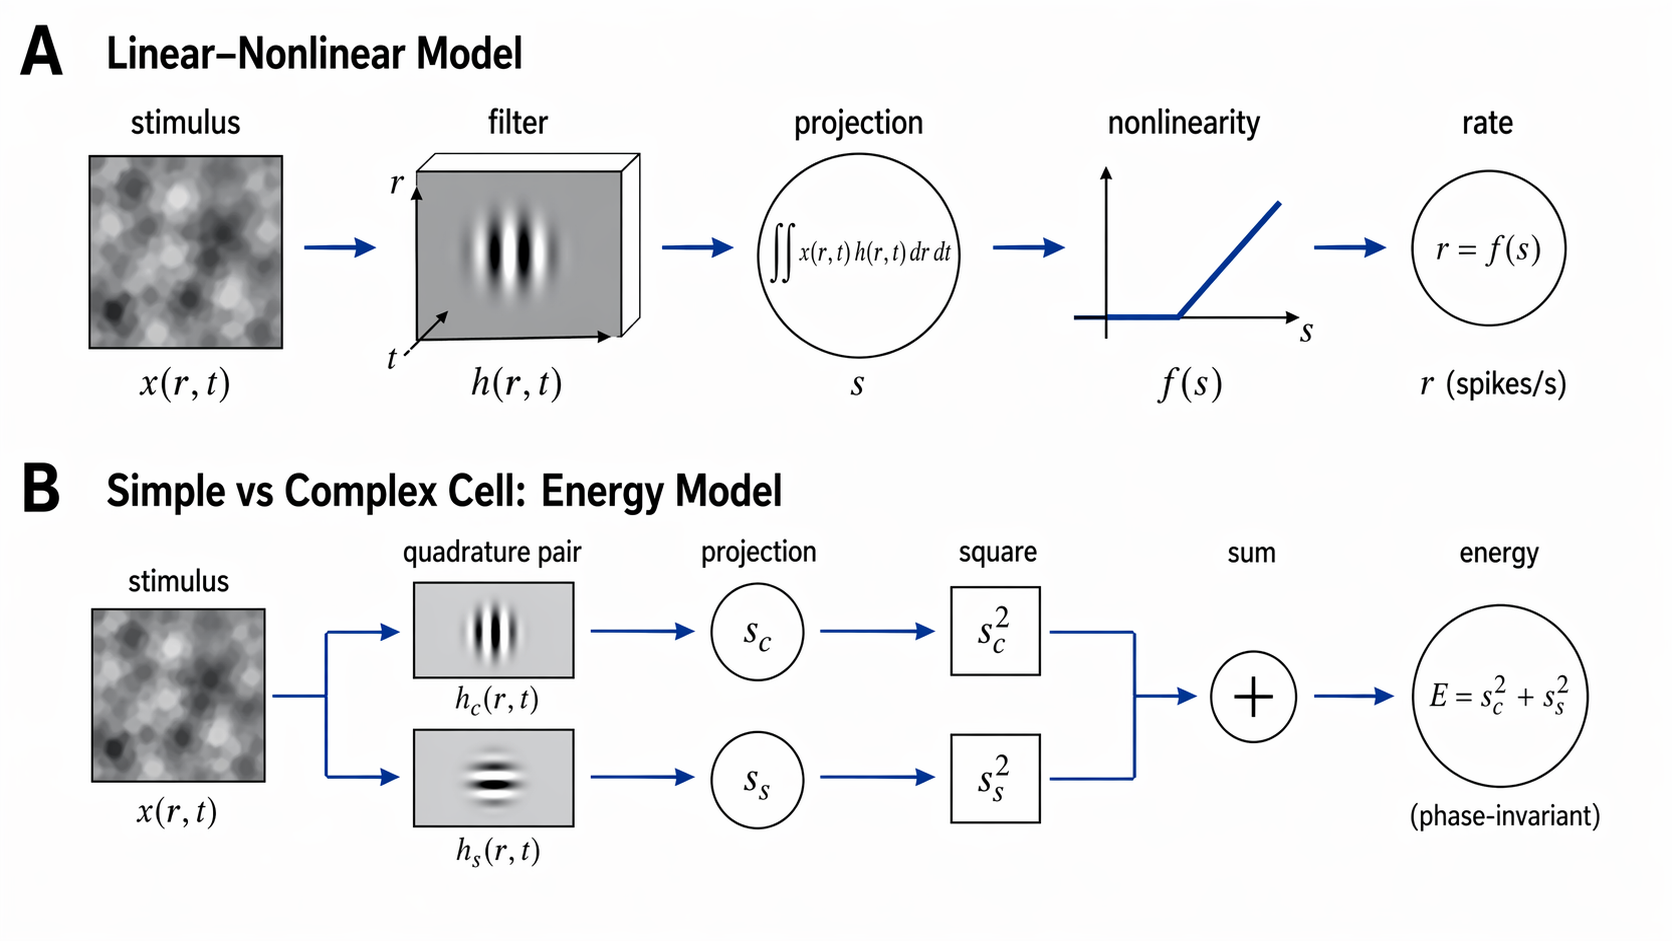
\includegraphics[width=\textwidth]{figures/mns-receptive-field-models.png}
\caption{Receptive-field computations. The LN model maps a stimulus to a scalar projection and then to a nonnegative rate; the energy model squares and sums a quadrature pair so orientation and frequency remain while phase is discarded.}
\label{fig:receptive-field-models}
\end{figure}

% ============================================================
\section{The Visual Hierarchy}
\label{sec:visual-hierarchy}
% ============================================================

The progression from retina to V1 illustrates a recurring theme in sensory neuroscience: successive stages of filtering and pooling build increasingly abstract representations.

Retinal ganglion cells and LGN neurons have center-surround receptive fields---roughly circular, with an excitatory center and inhibitory surround (or vice versa). These are not orientation selective; they respond to local contrast. V1 simple cells, by combining inputs from multiple LGN neurons with appropriately aligned receptive fields, create oriented filters. Complex cells, by pooling over simple cells, gain phase invariance. Each stage discards some information (phase, exact position) and preserves what matters for the next level of processing (orientation, spatial frequency, motion direction).

This hierarchy---from local contrast to oriented edges to phase-invariant features---is the computational backbone of early vision. Higher areas continue the pattern, building selectivity for texture, shape, and ultimately objects and faces, but those stages are beyond the scope of this chapter.


\begin{chaptersummary}

\begin{center}
\renewcommand{\arraystretch}{1.6}
\begin{tabularx}{\textwidth}{@{}l X X@{}}
  \toprule
  \textbf{Concept} & \textbf{Equation} & \textbf{Key Insight} \\
  \midrule
  Linear RF model &
  $\displaystyle L(t) = \int\!\!\int D\, s\;\dd x\,\dd y\,\dd\tau$ &
  Neuron as a linear filter (template matching) \\
  %
  Separability &
  $D(x,y,\tau) = D_s D_t$ &
  Space and time decouple \\
  %
  Gabor filter &
  Gaussian $\times$ cosine &
  Oriented, localized, band-pass spatial filter \\
  %
  Non-separability &
  $D(x,\tau) \neq D_s D_t$ &
  Required for direction selectivity \\
  %
  LN model &
  $r(t) = r_0 + F(L(t))$ &
  Rectifying nonlinearity fixes negative rates \\
  %
  Energy model &
  $E = L_1^2 + L_2^2$ &
  Quadrature pair $\Rightarrow$ phase invariance \\
  \bottomrule
\end{tabularx}
\end{center}

\end{chaptersummary}

\begin{conceptquestions}
  \item The linear receptive field model $L(t) = \int\!\!\int D\,s\;\dd x\,\dd y\,\dd\tau$ is a convolution. In plain language, what is this operation doing? Why is it sometimes called ``template matching''?

  \item What is the difference between the classical and non-classical receptive field of a neuron? How might the non-classical surround affect the neuron's response to a stimulus inside its classical receptive field?

  \item Explain what it means for a space-time receptive field to be \emph{separable}. If $D(x,y,\tau) = D_s(x,y)\,D_t(\tau)$, how does the response to a stimulus factor into spatial and temporal components?

  \item A simple cell has a separable space-time receptive field. A drifting grating and its reverse (same speed, opposite direction) are presented. Why does the cell respond identically to both? What would need to change for it to prefer one direction?

  \item The Gabor filter has parameters $k$ (spatial frequency), $\phi$ (phase), and $\sigma_x, \sigma_y$ (envelope widths). Describe what each parameter controls about the neuron's selectivity. What happens to spatial frequency selectivity if you narrow the Gaussian envelope?

  \item Why does a Gabor filter act as a band-pass filter in spatial frequency? What is the role of the Gaussian envelope versus the cosine component?

  \item A simple cell responds to a grating at its preferred orientation, spatial frequency, and phase. What happens to the response if you shift the grating by half a spatial period (a phase shift of $\pi$)? How does this compare to a complex cell?

  \item Why is the linear model insufficient on its own for predicting firing rates? What does the static nonlinearity $F$ need to do, and why is it called ``static''?

  \item The energy model predicts frequency doubling in complex cells. Show, using $\cos^2(\omega t) = \frac{1}{2}(1 + \cos 2\omega t)$, why the response to a counterphase grating modulates at twice the stimulus frequency.

  \item Hubel and Wiesel proposed that complex cells pool over simple cells with the same orientation preference but different phases. How does this relate to the mathematical structure of the energy model $E = L_1^2 + L_2^2$?

  \item Describe the visual hierarchy from retina to V1. What information is discarded at each stage, and what is preserved? Why is this progressive abstraction computationally useful?

  \item The temporal kernel of a V1 simple cell typically shows polarity reversal: the preferred polarity flips after roughly 50--100~ms. What does this reversal look like in the $x$-$\tau$ plot, and what is its functional significance?
\end{conceptquestions}
